\documentclass{article}
\usepackage[utf8]{inputenc}
\usepackage{commath}
\usepackage{graphicx}

\title{Iskanje po zbirski dokumentov -
        Latentno semantično indeksiranje \\
        \large Matematično modeliranje, projektna naloga}
\author{Nedžad Beus, Gašper Spagnolo, Tilen Ožbot}
\date{Junij 2022}

\begin{document}

\maketitle
\pagebreak

% PRVA STRAN
\section{Opis naloge}
\par Naloga je izdelati program, ki bo v zbirki dokumentov za dane ključne besede poiskal najbolj relevantne dokumente, s pomočjo metode \textit{latentnega semantičnega indeksiranja} (LSI). 
\par LSI je metoda za indeksiranje in iskanje, ki uporablja dekompozicijo singularnih vrednosti (SVD) za prepoznavanje vzorcev v odnosih med izrazi in pojmi v nestrukturirani zbirki besedil. Metoda temelji na načelu, da imajo besede, ki se uporabljajo v istem kontekstu, podoben pomen. Ključna značilnost LSI je, da lahko izlušči konceptualno vsebino besedila z vzpostavljanjem povezav med izrazi, ki se pojavljajo v podobnih kontekstih.

\subsection{Zahvale}
Zahvaljujemo se asistentu Damirju, ki nam je na govorilnih urah obrazlozil nekaj podrobnosti v zvezi s samo implementacijo naloge.

\newpage

\section{Resitev}
Nalogo razdelimo na več korakov:

\subsection{Izdelava začetne matrike}
Iz zbirke dokumentov zgradimo matriko A povezav med besedami in dokumenti. Vsakemu dokumentu v zbirki ustreza stolpec v matriki, vsaki besedi v zbirki pa vrstica. Element $a_{ij}$ naj v začetku predstavlja frekvenco \textit{i}-te besede v \textit{j}-tem dokumentu.

Za našo rešitev smo uporabili programski jezik \textit{Octave}. Octave obravnava besedilne dokumente kot enodimenzionalno matriko, katere člani so posamezne besede. Z iteracijo skozi to matriko (niz) bi odstranili ločila iz vsake besede in spremenili vse velike črke v male. 

Nato lahko preverimo, ali je beseda že prisotna v frekvenčni matriki, in če je tako, povečamo globalno in lokalno frekvenco te besede za $1$. Če beseda ni prisotna v frekvenčni matriki, dodajemo še eno vrstico v frekvenčno matriko pred povečanjem globalne in lokalne frekvence za $1$.

Če želimo obstoječi zbirki dodati nov dokument, lahko to naredimo z dopolnitvijo obstoječe frekvenčne matrike.



\textbf{Enostaven primer:}\\
Imejmo tri dokumente:

\begin{itemize}
    \item $d1:$ Jogurt je v vrecki.
    \item $d2:$ V vrecki imam jogurt.
    \item $d3:$ Zunaj piha veter.
\end{itemize}

Najprej prestejemo pojavitve besed v vseh dokumentih.

\[
\begin{tabular}{ |c|c|c|c| } 
    \hline
    beseda    & d1 &  d2  & d3\\
    \hline
    "jogurt"    & 1 & 1 & 0 \\ 
    "je"        & 1 & 0 & 0 \\ 
    "v"         & 1 & 1 & 0 \\ 
    "vrecki"    & 1 & 1 & 0 \\ 
    "imam"      & 1 & 0 & 0 \\ 
    "zunaj"     & 0 & 0 & 1 \\ 
    "piha"      & 0 & 0 & 1 \\ 
    "veter"     & 0 & 0 & 1 \\ 
    \hline
\end{tabular}
\]

Nato lahko zgradimo matriko $A$:

\[
A = \begin{bmatrix}
        1 & 1 & 0 \\
        1 & 0 & 0 \\
        1 & 1 & 0 \\
        1 & 1 & 0 \\
        1 & 0 & 0 \\
        0 & 0 & 1 \\
        0 & 0 & 1 \\       
        0 & 0 & 1 \\
 \end{bmatrix}
\]

\par Metodo in s tem rezultate lahko izboljšamo, če elemente matrike $a_{ij}$ izračunamo z bolj kompleksnimi merami kot so npr. entropija. Element matrike $a_{ij}$ lahko zapisemo kot
\[ a_{ij} = l_{ij} \cdot g_i,\]
kjer je $L_{ij}$ lokalna mera za pomembnost besede v dokumentu, $G_i$ pa globalna mera pomembnosti besede.
\[ L_{ij} = log(f_{ij} + 1)\]
\[ G_i = 1 - \sum_{j} \frac{p_{ij} log(p_{ij})}{logn} \]
\[ p_{ij} = \frac{f_{ij}}{gf_i},\]
kjer je $f_{ij}$ frekvenca \textit{i}-te besede v \textit{j}-tem dokumentu, $gf_i$ pa globalna frekvenca \textit{i}-te besede v bazi dokumentov. 
\par \textbf{Primer matrike $A$ z uporabo entropije:}
\[
A = \begin{bmatrix}
    1.6309  & 1.6309 &  0 \\
    1.0000  & 0      &  0 \\
    1.6309  & 1.6309 &  0 \\
    1.6309  & 1.6309 &  0 \\
    0       & 1.0000 &  0 \\
    0       & 0      &  1.0000 \\
    0       & 0      &  1.0000 \\
    0       & 0      &  1.0000 \\
 \end{bmatrix}
\]

\subsection{Razcep matrike}
\par Matriko A razcepimo z odrezanim SVD razcepom A = $U_kS_kV_k^T$, ki obdrži le \textit{k} največjih singularnih vrednosti. Stolpci matrike $U_k$ nam predstavljo t.i. vektorje izrazov, stolpci matrike $V_k$ pa t.i. vektorje dokumentov. S odstranjitvijo najmanjših singularnih vrednosti skušamo aproksimirati originalno matriko A in s tem zmanjšati šum. Število \textit{k} je odvisno od velikosti baze podatkov (npr. pri 1000+ dokumentih je \textit{k}=100 dobra aproksimacija).
\par \textbf{Primer razcepa matrike $A$ z uporabo entropije:}

\[
A = U \Sigma V^T
\]

\[
U = \begin{bmatrix}
    0.5601 &       0 & -0.0000 \\ 
   0.1717 &   0.0000 &  0.7071 \\
   0.5601 &        0 & -0.0000 \\
   0.5601 &        0 & -0.0000 \\
   0.1717 &  -0.0000 & -0.7071 \\
  -0.0000 &   0.5774 &  0.0000 \\
  -0.0000 &   0.5774 &  0.0000 \\
  -0.0000 &   0.5774 &  0.0000 \\
 \end{bmatrix}
\Sigma =
 \begin{bmatrix}
    4.1182 &        0 &        0 \\ 
        0  &   1.7321 &        0 \\
        0  &        0 &   1.0000 \\
 \end{bmatrix}
\]
\[
 V^T = 
 \begin{bmatrix}
     7.0711e^{-01} &   7.8505e^{-17} &  7.0711e^{01} \\ 
     7.0711e^{-01} &   1.9626e^{-16} & -7.0711e^{01} \\
   -2.3551e^{-16} &   1.0000         & -7.8505e^{-17} \\
 \end{bmatrix}
\]


\subsection{Vektor poizvedbe}
\par Besede po katerih želimo iskati oz. iskalni niz lahko zapišemo z vektorjem \textit{q}, ki je enake dolžine kot število vrstic v matriki A. Iskalni niz tretiramo kot dokument. Iz iskalnega niza generiramo vektor v prostoru dokumentov po naslednji formuli:
\[ \hat{q} = q^TU_kS_k^{-1},\]
ki jo izpeljemo iz naslednjih formul:
\[ A = USV^T,\]
\[ A^T = (USV^T)^T = VSU^T\]
\[ A^TUS^{-1} = VSU^TUS^{-1},\]
\[ V = A^TUS^{-1},\]
\[ \hat{q} = q^TUS^{-1}.\]
\par Dobljeni vektor $\hat{q}$ je v enakem prostoru kot stolpci v matriki $V_k$. Dokumenti oz. stolpci matrike $V_k$, ki najbolj ustrezajo poizvedbi so tisti, ki so dovolj blizu vektorju $\hat{q}$. Za razdaljo uporabimo kosinus kota med vektorjem. 
\[ cos(\alpha) = \frac{\hat{q} \cdot \Vec{v_i}}{\norm{\hat{q}} \cdot \norm{\Vec{v_i}}}\]

\textbf{Primer poizvedbe:}\\
Imejmo iskalni niz "imam jogurt", sestavimo iskalni vektor:
\[
\vec{q} = [1, 0, 0, 0, 1, 0, 0, 0]^T
\] Transformiramo vektor v prostor dokumentov:
\[
    \dot{q} =  [  1.7769e-01,   1.4731e-16,  -7.0711e-01]
\] Izracunamo se vektor posamicnega dokumenta:
\[
    \vec{d_1} = [ 7.0711e-01,   3.2374e-16,  -7.0711e-01]
\]
\[
    \vec{d_2} = [ 7.1486e-18,   1.0000e+00,   1.1776e-16]
\]
\[
    \vec{d_3} = [5.7189e-17,  -1.0000e+00,   7.3598e-17]
\] Nato izracunamo se pripadajoce kosinusne razdalje:

\[
 \begin{bmatrix}
    \vec{d_{q d_1}} \\ 
    \vec{d_{q d_2}} \\
    \vec{d_{q d_3}} \\
 \end{bmatrix} =
  \begin{bmatrix}
    -5.1345e-01 \\
    8.5812e-01 \\
    8.9575e-17 \\
 \end{bmatrix}
\]
Iz izracunanih vrednosti, lahko opazimo, da je dokument 2 najblizji poizvedovalnemu vektorju. Tam se tudi nahaja iskalni niz.
\newpage

\section{Dodajanje dokumentov in besed}
Predpostavimo, da je začetna matrika že zgrajena in SVD te matrike izračunan. Če želimo dodati nove dokumente oz. nove besede, obstajata dve možnosti za dodajanje:
\begin{enumerate}
    \item ponovno generiranje začetne matrike in izračunavanje SVD,
    \item metoda \textit{folding-in} ali zgibanje, ki je hitrejša.
\end{enumerate}
\subsection{Ponovno izračunavanje SVD}
 Za to možnost se odločimo, ko dodamo veliko število dokumentov oz. besed. Ponovno zgradimo začetno matriko in SVD razcep. Ponovni izračun SVD-ja omogoča, da nove besede in dokumenti neposredno vplivajo na latentno semantično strukturo, saj se ustvari nova začetna matrika in s tem drugačen SVD razcep. Slabost je, da ponovno izračunavanje SVD velike matrike zahteva veliko časa in pomnilnika.
\subsection{Metoda \textbf{folding-in} ali zgibanje}
\par Metoda zgibanja temelji na obstoječi latentni semantični strukturi, trenutni matriki, zato nove besede in dokumenti ne vplivajo na prestavitev ze obstoječih izrazov in dokumentov. Ta metoda zahteva manj časa in pomnilnika, vendar lahko poslabša prestavitev novih izrazov in dokumentov.
\par Postopek je enak postopku za vektor poizvedbe. Vsak nov dokument je predstavljen kot utežena vsota njegovih sestavnih vektorjev izrazov.
\[ \hat{d} = d^TU_kS^{-1}_k\]
Izračunan vektor je dodan naboru obstoječih vektorjev dokumentov ali stolpcev v matriki $V_k$. \\

% slika
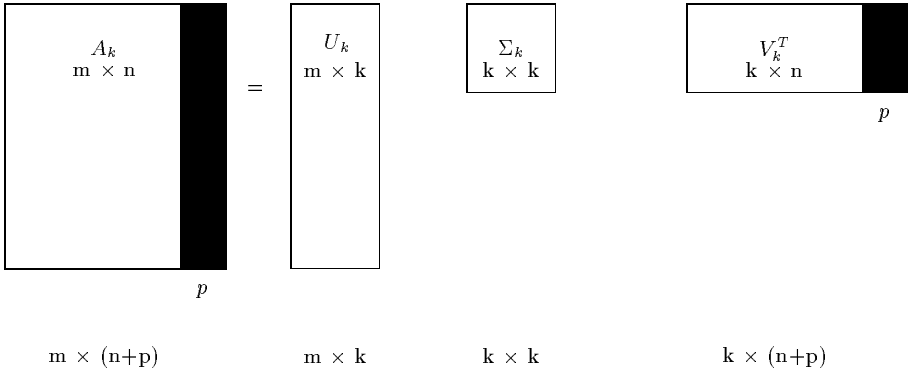
\includegraphics[scale=0.5]{./assets/zaDokumente.png}
\\
\par Podobno lahko nove besede izrazimo kot uteženo vsoto vektorjev dokumentov, v katerih se pojavljajo.
\[ \hat{t} = tV_kS^{-1}_k\]
Izračunani vektor je dodan naboru obstoječih vektorjev besed ali stolpcev v matriki $U_k$. \\

% slika
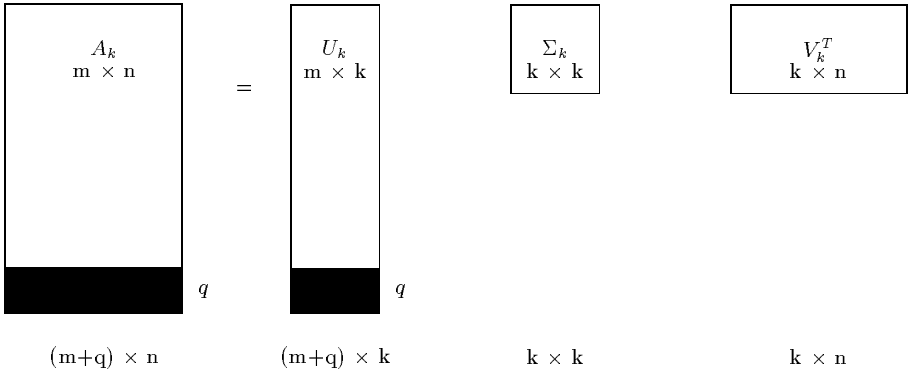
\includegraphics[scale=0.5]{./assets/zaTermine.png}
\newpage

\section{Rezultati}
Za bazo podatkov smo se odločili za recepte jedi. Testirali smo nad 260 dokumenti in dobili presenetljive rezultate. Metoda je bila zelo ušpesna in našla pravilne rezultate. Med testiranjem smo tudi opazovali kako se spreminjajo iskalni rezultati, v primeru, da spremenimo število uporabljenih lastnih vrednosti. Izkazalo se je da smo že pri 50 lastnih vrednosti dobili dovolj natančne rezultate.


\subsection{Primerjava glede na število uporabljenih lastnih vrednosti}
Ker vemo, da je SVD razcep računsko drag, nas je zanimalo, koliko poračunanih lastnih vrednosti je dovolj (glede na naše testne primere, pri 260 dokumentih), da še vedno dobimo zadvoljive rezultate, pri hitrem razcepu. Tako zmanjšamo komputalno moč
in prostor, katerega bi porabili za shranjevanje matrike A, tako je lahko matrika A cel čas v hitrem pomnilniku, in ne potrebujemo dosegati vrednosti iz diska, to bi bilo zelo pčasno.
Na grafih je z zeleno barvo označena "naivna" metoda, z modro pa "izboljšana" metoda, Na x-osi, je predstavljena številka dokumenta (prvih 10 dokumentov), na y-osi pa je prikazana moč iskalnega niza(kosinusna razdalja).

\subsubsection{20 singularnih vrednosti}

Najprej smo poskušali s 20imi lastnimi vrednostm, takoj lahko opazimo ogromne razlike med "naivno" in "izboljšano" metodo.

\textit{Spomnimo se: "Naivna" metoda samo prešteje pojavitve posameznih besed glede na dokument, "izboljšana" metoda pa s pomočjo globalnih in lokalnih frekvenc izboljša matriko A }

\begin{small}
\begin{verbatim}
Enter search query: milk
Naive method:
ans =

   105.0000     0.6526
   244.0000     0.5159
   233.0000     0.4677
    56.0000     0.4554
   216.0000     0.4466
    47.0000     0.4430
    37.0000     0.4419
   138.0000     0.4341
   218.0000     0.4270
     4.0000     0.4176

Better method:
ans =

   105.0000     0.7556
     4.0000     0.5751
   106.0000     0.5650
    72.0000     0.4830
   145.0000     0.4750
   109.0000     0.4723
   187.0000     0.4369
   244.0000     0.4357
   216.0000     0.4310
   177.0000     0.4192    
\end{verbatim}
\end{small}

\begin{center}
    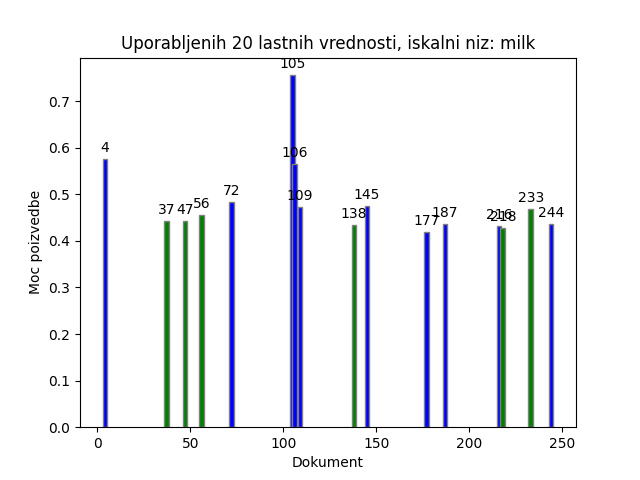
\includegraphics[scale=0.65]{../graphs/generated_graphs/graph_20_singular_values_used.png}    
\end{center}


Iz grafa lahko opazimo, da se metodi, v najdenih dokumentih precej razlikujejo. Če pogledamo vsebino dokumenta 105, opazimo pojavitev niza milk. Kar nam daje vzpodbudne rezultate, vendar zal dokumentov, ki 
bi jih zeleli ni na seznamu (taksnih, ki imajo veliko vec pojavitev iskalnega niza)
\begin{verbatim}
Cheesy Potato Bake
.......................
After 2 min or bubbly remove from heat
Add milk slowly, stirring constantly
.......................
Put in oven for 45 min. If it starts to brown too much cover with tinfoil.
\end{verbatim}


\subsubsection{50 singularnih vrednosti}

\begin{small}
\begin{verbatim}
Enter search query: milk
Naive method:
ans =

    59.0000     0.5884
   244.0000     0.4946
   216.0000     0.4717
   177.0000     0.4398
   106.0000     0.4022
   109.0000     0.3938
   104.0000     0.3926
   192.0000     0.3291
   218.0000     0.3212
   199.0000     0.2908

Better method:
ans =

   133.0000     0.4610
   244.0000     0.4547
   104.0000     0.3921
   216.0000     0.3719
   199.0000     0.3715
   106.0000     0.3709
   189.0000     0.3558
   218.0000     0.3493
    59.0000     0.3378    
\end{verbatim}
\end{small}

\begin{center}
    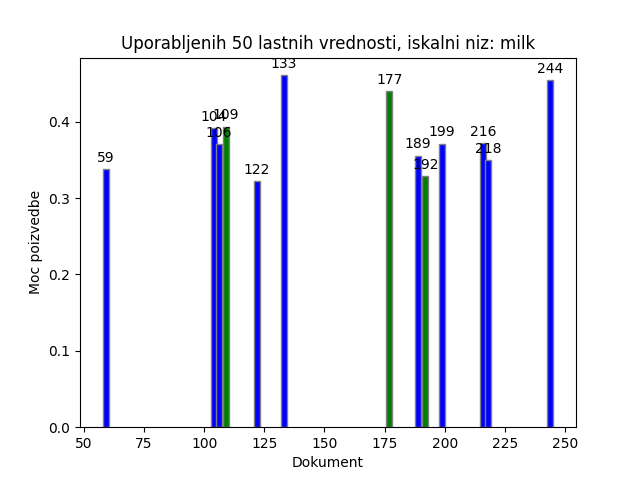
\includegraphics[scale=0.65]{../graphs/generated_graphs/graph_50_singular_values_used.png}
\end{center}

Iz grafa lahko opazimo, da sta obe metodi zelo izboljšani, dobimo tudi ze prekrivanja med stolpci.
Naivna metoda nam kot prvi dokument vrne 59, poglejmo vsebino:
\begin{verbatim}
Torrijas
Mull the milk with cinnamon and a bit of sugar (not too much, the milk is already sweet). Add the lemon rind if you want.
Cool down the milk.
While the milk is cooling, beat the eggs and heat up half a pan of olive oil.
Cut the dry bread in slices. Soak it in the milk.
Coat the bread soaking it in the beaten eggs.
Fry the soaked & coated bread with the heated oil.
Optionally sprinkle some sugar onto the Torrijas.
Enjoy when they are cooled down. Don’t eat too much, it won’t be easy resisting!
\end{verbatim}
Metoda deluje! V dokumentu smo našteli kar 5 pojavitev iskalnega niza.

Izboljšana metoda nam kot prvi dokument vrne 133, poglejmo vsebino:
\begin{verbatim}
Swedish Pancakes
At medium/low heat begin melting the butter, and continue with beating eggs in large bowl, add salt, sugar, milk, flour and mix.
Add melted butter while stirring batter.
... dolg dokument ...
of your choice.
\end{verbatim}
Oh to je pa čudno! Samo eno pojavitev iskalnega niza smo dobili. Tukaj se pokaze, glavna lastnost LSI, saj LSI ni namenjen za iskanje po ključnih vrednostih, temveč povezuje tudi pomen besede. Vendar 
je sama beseda dovolj, za preverjanje kako se metoda obnaša in ali se sploh pravilno obnaša.

Pri 50-ih lastnih vrednostih so rezultati ze zadovoljvi, vendar nas iz "firbca" zanima, kaj se zgodi, ce povečamo število uporabljenih lastnih vrednosti na 80.

\subsubsection{80 singularnih vrednosti}

Poizvedba:
\begin{small}
\begin{verbatim}
    Enter search query: milk
Naive method:
ans =

    59.0000     0.6804
   244.0000     0.4541
    36.0000     0.4271
   177.0000     0.3887
   141.0000     0.3697
   218.0000     0.2942
    40.0000     0.2840
   216.0000     0.2796
    49.0000     0.2737
   106.0000     0.2728

Better method:
ans =

    59.0000     0.4751
   244.0000     0.3838
    36.0000     0.3781
   141.0000     0.3773
    40.0000     0.3559
   133.0000     0.3009
   182.0000     0.3009
   106.0000     0.2714
   181.0000     0.2664
   218.0000     0.2616
\end{verbatim}
\end{small}

\begin{center}
    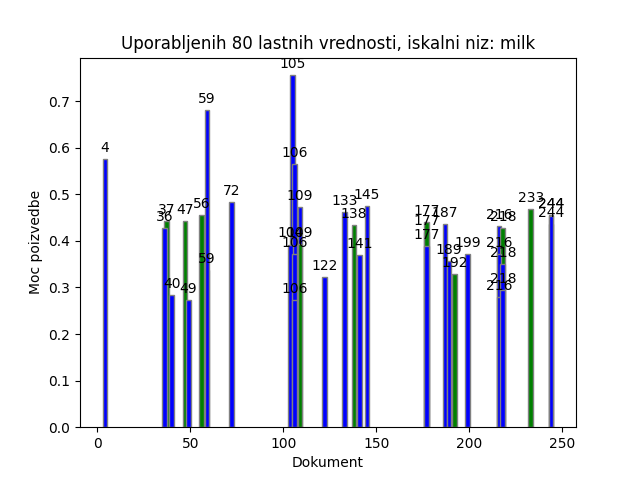
\includegraphics[scale=0.65]{../graphs/generated_graphs/graph_80_singular_values_used.png}   
\end{center}

Zanimv graf! Kaj se je zgodilo? Lahko opazimo, da nam obe metodi vrneta vseh prvih 10 dokumentov, ki so enaki, vendar z različno močjo. Iz tega dejstva lahko sklepamo, da je uporaba entropije dejansko
zelo pripomogla k zmanjšanju uporabe lastnih vrednosti, pri zgradbi matrike! 
Obe metodi nam vrneta dokument 105 z najvišjo močjo, poglejmo kaj se nahaja v dokumentu:
\begin{verbatim}

\end{verbatim}
Z obema metodama smo pridobili zelo dobre rezultate! V vseh najdenih dokumentih, se nahaja nas iskalni niz.
\newpage

\section{Zakljucek}
Glede na teste v prejsnem razdelku, smo z naivno metodo pridobili zadovoljive rezultate z uporabo 80ih lastnih vrednosti. Z izboljšano metodo, pa je dovolj ze 50 lastnih vrednosti, kar se nam zdi
odličen dosežek! Seveda to velja samo za nase testne primere, v praksi se število uporabljenih lastnih vrednosti lahko zelo razlikuje; potrebno je testirati.

Resitev, pripravo testov in izris grafov, najdete na naslednji povezavi: 
\begin{verbatim}
    https://github.com/vekejsn/mm-projekt
\end{verbatim}
\newpage

\section{Viri in literatura}
\begin{enumerate}
    \item  M. W. Berry, S.T. Dumais, G.W. O’Brien, Michael W. Berry, Susan T.
    Dumais, and Gavin. Using linear algebra for intelligent information retrieval.
    SIAM Review, 37:573–595, 1995.
    \item Susan T. Dumais. Improving the retrieval of information from external 
    sources. Behavior Research Methods, Instruments, \& Computers, 23(2):229–
    236, 1991.
\end{enumerate}
\end{document}


